\documentclass{seminar}
%\documentclass[article]{seminar}

\pagestyle{empty}

\usepackage{psfig}
\usepackage{fancybox}
\usepackage{epsfig}
\usepackage{epic}
\usepackage{eepic}
\usepackage{subfigure}

\usepackage{latexsym}
\usepackage{graphicx}
\usepackage{bar}

\newcommand{\cA} {\mbox{$\cal A$}}
\newcommand{\cB} {\mbox{$\cal B$}}
\newcommand{\cD} {\mbox{$\cal D$}}
\newcommand{\cF} {\mbox{$\cal F$}}
\newcommand{\cI} {\mbox{$\cal I$}}
\newcommand{\pg}  {\overline{g}}
\newcommand{\tc}  {T_{\Omega}}
\newcommand{\tck}  {T_{\Omega}}
\newcommand{\tckk} {T_{\Omega}}
\newcommand{\tcc} {T_{\Omega}}
%\newcommand{\tc}  {T_{\Omega,x}}
%\newcommand{\tck}  {T_{\Omega,x_{k}}}
%\newcommand{\tckk} {T_{\Omega,x_{k+1}}}
%\newcommand{\tcc} {T_{\Omega,x^*}}

\usepackage{colordvi}
\newcommand{\RED} {\BrickRed}
\newcommand{\REDBALL}{\item[\RED{$\bullet$}]}
\newcommand{\REDDIAMOND}{\item[\RED{$\diamond$}]}
\newcommand{\REDEXAMPLE}{\item[\RED{Ex:}]}
\newcommand{\REDSTAR}{\item[\RED{$\star$}]}
\newcommand{\REDCIRC}{\item[\RED{$\circ$}]}
\newcommand{\REDPLUS}{\item[\RED{+}]}
\newcommand{\REDMINUS}{\item[\RED{--}]}
\newcommand{\REDQUESTION}{\item[\RED{?}]}
\newcommand{\REDEXCLAIM}{\item[\RED{!}]}
\newcommand{\REDRIGHTARROW}{\item[\RED{$\Rightarrow$}]}

% My modifications to the list environment
\newcommand{\jti}{\begin{itemize}%
{\setlength{\itemsep}{0 pt}\setlength{\topsep}{0 pt}
\setlength{\partopsep}{0 pt}}}

\newcommand{\ejti}{\end{itemize}}

\newcommand{\heading}[1]{%
  \begin{center}
    \large\bf
    \shadowbox{\RED{#1}}%
  \end{center}
  \vspace{1ex minus 1ex}}

\newcommand{\twolineheading}[2]{%
  \begin{center}
    \large\bf
    \shadowbox{\RED{#1}\\
        \RED{#2} }%
  \end{center}
  \vspace{1ex minus 1ex}}

\newcommand{\picheading}[2]{%
  \begin{center}
    \large\bf
    \shadowbox{\RED{#1}}%
  \end{center} 
  \vspace{-0.5in}
  \hfill \epsfig{figure=#2,height=0.5in}        
  \vspace{1ex minus 1ex}}

\begin{document}

\slideframe{none}
\begin{slide}
\centering
{\Large  A Limited Memory Variable Metric Method for
Bound Constrained Optimization
}

\vspace{.5in}

\begin{minipage}{0.5\linewidth}
\vspace{0.4in}
\centering
{\sc Steven J. Benson} \\
% {\tt benson@mcs.anl.gov}\\

\vspace{0.125in}
{\sc Jorge Mor\'e}

\vspace{0.125in}
\small
Argonne National Labs \\
Math and Computer Science Division \\

\vspace{0.125in}
\end{minipage} \hfill
\begin{minipage}{0.4\linewidth}
\centering
\vspace{0.25in}
\psfig{figure=/home/benson/logos/argonne.eps,height=1.4in,width=1.4in}
\end{minipage}

\end{slide}

\begin{slide}
\heading{Nonlinear Problem with Bound Constraints}
\centering
\[
\min \{ f(x) : l \leq x \leq u \} ,
\]

\vspace{0.25in}

\begin{minipage}{0.6\linewidth}

\jti
\REDBALL $ x \in \Re^{n}$
\REDBALL $ l,u \in \Re^{n}$ are fixed
\REDBALL $f : \Re^n \mapsto \Re $ is a nonlinear function 
whose gradient $\nabla f$ is available
\ejti

\end{minipage} \hfill
\begin{minipage}{0.35\linewidth}
\centering
\psfig{figure=cube.eps,height=1.0in,width=1.2in}
\end{minipage}

\end{slide}


\begin{slide}
\heading{Projected Gradient}
Exact and approximate solution can be defined using the
projection operator $ \tc $
\begin{equation} \label{projection-tangent}
 \left[ \tc d \right] _i = \left\{
\begin{array}{lll}
d_i & \mbox{ if } & x_i \in (l_i, u_i) \\
\min \{ d_i,0 \} & \mbox{ if } & x_i = l_i \\
\max \{ d_i,0 \} & \mbox{ if } & x_i = u_i
\end{array}
\right.
\end{equation}

\vspace{0.25in}

\jti
\REDBALL A solution $x^*$ satisfies $\tcc \nabla f(x^*) =0$.
\REDBALL Approximate solutions satisfy $\| \tc \nabla f(x) \| \leq \tau$ .
\ejti

\end{slide}


\begin{slide}
\heading{Unconstrained BFGS method}

Use gradient vectors to compute an approximate inverse Hessian.

Let $H_{k+1}$
\[ \mbox{minimize } \| H - H_k \|_{W} \]
subject to 
\jti
\REDBALL $ H=H^T$ \hspace{2.1in} (Symmetry)

\REDBALL $H y_{k} = s_{k}$ \hspace{1.8in} (Secant Equation)

\REDBALL $s_{k} = x_{k+1} - x_{k}$, \hspace{0.2in} $y_{k} = \nabla f(x_{k+1}) - \nabla f(x_{k})$


\ejti

{\tiny
$\| A \|_{W} = \| W^{1/2} A  W^{1/2} \|_{F}$ for any 
matrix $W$ satisfying $W y_{k} = s_{k}$.
%$W y_k = s_k$.
}

\end{slide}

\begin{slide}
\heading{Unconstrained BFGS matrix update}

\jti
\REDBALL Setting  $s_k = x_{k+1} - x_{k}$ and
$y_k= \nabla f(x_{k+1}) - \nabla f(x_{k})$,

\[ H_{k+1} = V_{k}^T H_{k} V_{k} + \rho_k s_{k} s_k^T \]
where 
\begin{equation}\label{defrho}
\rho_k = \frac{1}{\langle y_k, s_k \rangle} \hspace{0.5in} \hbox{ and } \hspace{0.5in} V_k = I - \rho_k y_k s_k^T. 
\end{equation}

\REDBALL $H_{k+1} \succ 0$
if $H_0 \succ 0,$ and $\rho_k > 0.$
\ejti


\end{slide}

\begin{slide}
\heading{Limited Memory BFGS method}

To reduce the high storage and
computational costs on large problems, the L-BFGS method stores a 
limited number of correction pairs $\{ s_i, y_i\}$,
$i = k-m+1, \ldots, k$. 

\begin{equation}\label{lbfgs}
\begin{array}{ll} 
H_k = &\left( V_{k-1}^T \ldots  V_{k-m}^T \right) H_k^0 \left( V_{k-m} \ldots  V_{k-1} \right) \hspace{0.05in} + \\
& \rho_{k-m} \left( V_{k-1}^T \ldots  V_{k-m+1}^T \right) s_{k-m} s_{k-m}^T  \left( V_{k-m+1} \ldots  V_{k-1} \right) \hspace{0.05in} + \\
& \ldots \hspace{0.05in} + \\
& \rho_{k-2} \left( V_{k-1}^T \right) s_{k-2} s_{k-2}^T  \left( V_{k-1} \right) \hspace{0.05in} + \\
& \rho_{k-1} s_{k-1} s_{k-1}^T.
\end{array}
\end{equation}

\end{slide}

\begin{slide}
\heading{Two Loop Recursion}

To compute $\hat d := H_k v$,

\jti
\REDBALL  $\hat d \leftarrow  v$
\REDBALL  for $i=k-1, \ldots, k-m $

\jti
\REDBALL  $\beta_i \leftarrow { \rho_i}{\langle \hat d, s_i \rangle } ;$
\REDBALL  $\hat d \leftarrow \hat d - \beta_i y_i;$
\ejti

\REDBALL $\hat d \leftarrow H_k^0 \hat d ;$

\REDBALL for $i= k-m, \ldots, k-1$
\jti
\REDBALL  $\hat d \leftarrow \hat d + \left( \beta_i - { \rho_i }{ \langle \hat d , y_i \rangle 
} \right) s_i $
\ejti

\ejti

\end{slide}

\begin{slide}
\heading{Bound Constrained Optimization}

If we impose bounds, $l \leq x \leq u$, then 
many methods for unconstrained optimization can be adapted for
bound constrained optimization methods.

\jti

\REDBALL Projected gradient methods adapt the steepest descent 
\REDBALL Newton method like TRON apply unconstrained minimization
techniques to a sequence of faces.
\REDBALL BFGS Method

\ejti

\end{slide}


\begin{slide}
\heading{L-BFGS-B}
Proposed by Byrd, Lu, Nocedal, Zhu

\jti
\REDBALL Uses compact ( or outer product ) form of L-BFGS matrix instead
of the two-loop recursion form.

\REDBALL Use gradient projection to select a set of free variables ${\cal F}$

\REDBALL 
Let $\hat H = Z^T H Z$ and $\hat g = Z^T \nabla f$

\REDBALL Solve $\hat H  \hat d = \hat g$
\[ x_{k+1} = \hat x - \alpha d_k. \]
\ejti

\end{slide}

\begin{slide}
\heading{Definition}
%\begin{definition}\label{D1}
For any subset $\cF$ of variables in $\Re^n$, let
$p$ denote the cardinality of $\cF$ and let
$Z : \Re^n \mapsto \Re^p$ be a matrix whose columns are unit vectors
(i.e.~rows of the identity matrix) that span $\Re^p$.  
That is, $Z = \left[ e_i \right]_{i \in \cF}$.
Given a symmetric positive definite matrix 
$\overline{H}_k \in \Re^{p \times p}$ 
and a correction pair
$\{ \overline{s}_k , \overline{y}_k \} $ such that
$\overline{s}_i = Z^T \left( x_{k+1} - x_k \right) $,
$\overline{y}_i = Z^T ( \nabla f(x_{k+1}) - \nabla f(x_k) ) $, 
and
$\overline{\rho}_{i} = 1 / \langle \overline{y}_i, \overline{s}_i \rangle > 0$,
define the
{\bf reduced L-BFGS matrix on the set $\cF$}, $\overline{H}_{k+1}$,
to be the solution to the problem
\[
\begin{array}{ll}
\min & \| \overline{H} - \overline{H}_k \|_W \\
\mbox{such that} & \overline{H} = \overline{H}^T \mbox{ and } 
\overline{s}_k = \overline{H} y_k \\
\end{array}
\]

%\end{definition}

\end{slide}

\begin{slide}
\heading{Example}
\[
\min   f(x_1,x_2,x_3) =  x_1^2 - x_1 x_2  + 0.75 x_2^2 + 0.5 x_3^2 + 4 x_1 - 4 x_2 - 2 x_3 : x_3 \geq 0 ,
\]
\jti
\REDBALL Unique minimum at $(0, 8/3, 2)$.
\REDBALL The optimal face is $ \{ (x_1,x_2,x_3) : x_1 = 0; \} $
\REDBALL 
$ \nabla f = [ 2 x_1 - x_2 + 4, -x_1 + 1.5 x_2 - 4 , x_3  - 2  ]^T $
\REDBALL
$\nabla f(0,0,0) = [ 4, -4, -2]^T, 
\hspace{0.25in}
\nabla f(0,2,1) = [ 2, -1 , -1]^T
$
\ejti

\end{slide}

\begin{slide}
\heading{BFGS in a Subspace}

Fix $x_1=0$. Consider the unconstrained problem in $x_2$ and $x_3$.
Start the BFGS algorithm at the origin, 
step in the direction of the gradient to
where $x_2=2$ and $x_3=1$.  If $\overline{H}_0 = \overline{I}$, then
$\overline{y}_0 = [3, 1]^T$ and $\overline{s}_0 = [2, 1]^T$, and
\[
\overline{H}_1 =  
\left[
\begin{array}{cc}
33/49  & -1/49   \\
-1/49  &  52/49  \\
\end{array}
\right]
\]
and the step direction
\[
\overline{H}_1 [ -1 , -1 ]^T = [ -32/49 , -51/49 ]^T.
\]

\end{slide}

\begin{slide}
\heading{L-BFGS-B direction}
Now let $H_0 = I$ and consider a full space matrix $H_1$.  
Start at the origin at step in the direction of the
projected gradient to  $x_1=0$, $x_2=2$ and $x_3=1$.
The correction pairs:
\[
y = [-2, 3, 1]^T;  \hspace{1in} s = [ 0, 2, 1]^T
\]
produce the BFGS matrices.
\[
H_1 =
\left[     
\begin{array}{ccc}
1     & 4/7   &  2/7 \\
4/7  &  1    &  1/7 \\
2/7  &  1/7  &  8/7 \\
\end{array}
\right],
\]
The step directions 
$\overline{H}_1 [ -1 , -1 ]^T = [ -8/7, -9/7]^T$

\end{slide}

\begin{slide}
\heading{L-BFGS-B}

%\begin{lemma} \label{L1}
Let $x_{k-m}, \ldots, x_{k}$ lie on the optimal face and
denote $\overline{H}_k$ as the reduced L-BFGS matrix on the set
of free variables at $x_k$.
If there exist $i$,  ($k-m \leq i \leq k-1$), such that
$Z Z^T y_i \neq y_i$,
then
\[  Z^T H_k Z \neq \overline{H}_k \]
and
\[ [Z^T H_k Z] [Z^T \nabla f(x_k)] \neq \overline{H}_k [ Z^T \nabla f(x_k)]. \]

%\end{lemma}

\end{slide}


\begin{slide}
\heading{Another bound constrained BFGS method}

Let $H_{k+1}$
\[ \mbox{minimize } \| H - H_k \|_{W} \]
subject to 
\jti
\REDBALL $ H=H^T$

\REDBALL $H y_{k} = s_{k}$

\REDBALL $s_{k} = x_{k+1} - x_{k}$, \hspace{0.2in} $y_{k} = \tckk f(x_{k+1}) - \tck f(x_{k})$

\ejti

{\tiny
$\| A \|_{W} = \| W^{1/2} A  W^{1/2} \|_{F}$ for any 
matrix $W$ satisfying $W y_{k} = s_{k}$.
%$W y_k = s_k$.
}

\end{slide}

\begin{slide}
\heading{Bound constrained BFGS matrix update}

\jti
\REDBALL Set  $s_k = x_{k+1} - x_{k}$ and
$y_k= \tckk \nabla f(x_{k+1}) - \tck \nabla f(x_{k})$,

\[ H_{k+1} = V_{k}^T H_{k} V_{k} + \rho_k s_{k} s_k^T \]
where 
\begin{equation}\label{defrho2}
\rho_k = \frac{1}{\langle y_k, s_k \rangle} \hspace{0.5in} \hbox{ and } \hspace{0.5in} V_k = I - \rho_k y_k s_k^T. 
\end{equation}

\REDBALL $H_{k+1} \succ 0$
if $H_0 \succ 0,$ and $\rho_k > 0.$
\ejti

The L-BFGS matrix structure and two loop recursion also apply.

\end{slide}



\begin{slide}
\heading{BLMVM}
Update the L-BFGS matrix using projected gradients

Set 
\[ x_{k+1} = P [ x_k - \alpha_k H_k \nabla f(x_k) ] \]
for an appropriate stepsize $\alpha_k$.

\[ P(x) = {\rm mid} (l,u,x) \]

\end{slide}

\begin{slide}
\heading{BLMVM}

%\begin{lemma} \label{L1}
Let $\overline{H}_k$ be the reduced L-BFGS matrix on the set
of nonbinding variables at $x_k$.
If
\begin{enumerate}
\item[(i)]   $x_{k-m}, \ldots, x_{k}$ lie on the same face, and
\item[(ii)]  $\cB (x_{k-m}) = \ldots = \cB (x_{k}) = \cB (x^*)$, 
\item[(iii)]  $Z^T H^0_k d = \overline{H}^0_k Z^T d$ for all $d \in \Re^n$, 
\end{enumerate}
then
\[  Z^T H_k Z = \overline{H}_k \]
and
\[ Z^T H_k \nabla f(x_k) = \overline{H}_k Z^T \nabla f(x_k). \]
%\end{lemma}

\end{slide}

\begin{slide}
\heading{Example}
\[
\min   f(x_1,x_2,x_3) =  x_1^2 - x_1 x_2  + 0.75 x_2^2 + 0.5 x_3^2 + 4 x_1 - 4 x_2 - 2 x_3 : x_3 \geq 0 ,
\]
\[
\tck \nabla f(0,0,0) = [ 0, -4, -2]^T,
\hspace{0.5in}
\tck \nabla f(0,2,1) = [ 0, -1 , -1]^T,
\]

Let
\[ y = [ 0,3,1];  \hspace{0.4in} s = [0,2,1]; \]


\[ H_1 = \left[
\begin{array}{ccc}
1 &  0 &  0 \\
0 &  33/49  & -1/49   \\
0 &  -1/49  &  52/49  \\
\end{array}
\right] 
\]
$H_1 \nabla f(0,2,1)^T = [ 2, -32/49 , -51/49 ]^T.$
SAME as BLMVM in subspace!
\end{slide}


\begin{slide}
\heading{Possible difficulties}

\jti
\REDBALL We must check the descent direction.  
If $ \langle \tck  H_k \nabla f(x_k), \nabla f(x_k) \rangle \leq 0$,
let $ x_{k+1} = P [ x_k - \alpha_k \nabla f(x_k)].$
\REDBALL
Since there is no equivalent of the Wolfe conditions for bound
constrained optimization, a line search cannot enforce condition 
that $\langle s_k, y_k \rangle >0 $.  In this event, skip the matrix update.

\ejti

\end{slide}


\begin{slide}
\heading{Test Problems}
Computations tests were performed using
\jti
\REDBALL Bound constrained problems in MINPACK-2
\REDBALL Systems of nonlinear equations in MINPACK-2
\REDBALL Bound constrained problems in CUTE collection
\ejti

\vspace{0.25in}

On the optimization problems,
both codes
were terminated when
\[ \| \tck \nabla f(x_k) \| \leq  \mbox{min}\{ 10^{-5}, 10^{-10} |f(x_k)| \}. \]

For the nonlinear equations, the solvers were terminated when
the objective function was less the $10^{-4}$.

\end{slide}


\begin{slide}
\heading{BLMVM v. L-BFGS-B (Function Evaluations)}
\begin{figure}[ht]
\begin{center}
%\caption{BLMVM v. L-BFGS-B. (Function Evaluations) }
\includegraphics[width=0.8\textwidth,height=0.58\textwidth]{h2.eps}
% \psfig{figure=cube.eps,height=3.0in,width=4.0in}
\end{center}
\end{figure}
\end{slide}



\begin{slide}
\heading{BLMVM and L-BFGS-B (Time)}
\begin{figure}[ht]
\begin{center}
%\caption{Comparson of BLMVM and L-BFGS-B. (Time) }
\includegraphics[width=0.8\textwidth,height=0.58\textwidth]{h1.eps}
% \psfig{figure=cube.eps,height=3.0in,width=4.0in}
\end{center}
\end{figure}
\end{slide}

\begin{slide}
\heading{Parallel Implementation}
\centerline {\includegraphics[width=1.0\textwidth,height=2.5in]{surf5.ps}}
\end{slide}

\begin{slide}
\heading{Performance of BLMVM on Obstacle Problem}

\begin{table}[bhpt]
\small
\begin{center}
\begin{tabular}{|cccccc|}
\hline
\multicolumn{1}{|c|}{Processors} &
\multicolumn{1}{c|}{BLMVM} &
\multicolumn{1}{c|}{Execution} &
\multicolumn{3}{c|}{Percentage of Time} \\
%\multicolumn{1}{|c|}{} \\
\multicolumn{1}{|c|}{Used}&
\multicolumn{1}{|c|}{Iterations}&
\multicolumn{1}{c|}{Time}&
\multicolumn{1}{c}{AXPY}&
\multicolumn{1}{c}{Dot} &
\multicolumn{1}{c|}{FG} \\
%\multicolumn{1}{c|}{FLOPS} \\
\hline

8 & 996 & 1083.8 & 31  & 9 & 61 \\ %& 256 \\
16 & 991 & 538.2 & 30 & 10 & 61 \\ %& 580 \\
32 & 966 & 267.7 & 29 & 11 & 60 \\ %& 1137 \\
64 & 993 & 139.5 & 27 & 12 & 60 \\ %& 2027 \\
128 & 987 & 72.4 & 25 & 15 & 60 \\ %& 3728 \\
256 & 996 & 39.2 & 26 & 18 & 55 \\ %& 8009 \\
512 & 1000 & 21.6 & 23 & 22 & 53 \\
\hline
\end{tabular}
%\caption{Performance of BLMVM on Obstacle Problem.}
\label{routines}
\end{center}
\end{table}

\end{slide}

\begin{slide}
\heading{Scalability of BLMVM and Obstacle Problem}
\begin{figure}[ht]
\begin{center}
%\caption{Scalability of BLMVM on the Obstacle Problem.}
   \subfigure[Overall Efficiency]{
   \label{G14}
   \includegraphics[width=0.45\textwidth,height=0.4\textwidth]{f4.eps}}
   \hskip 0.00\textwidth
   \subfigure[Floating Point Efficiency]{
   \label{G14chol}
   \includegraphics[width=0.45\textwidth,height=0.4\textwidth]{f3.eps}} \\
\label{figure2}
\end{center}
\end{figure}

\end{slide}

\end{document}


